%!TEX root = ../physical-olympics-2.tex
\chapter{振动与波}


\section{方程与谐振}

\subsection{简谐振动的定义}
振动是最常见的物理现象.\,而振动中的最简单(simple)而和谐(harmonic)者谓之\emph{简谐振动}(simple harmonic oscillation).\,对\emph{谐振子}(harmonic oscillator)的学习与研究是会贯彻整个物理理论不同层次内容的始终的.\,现在是经典力学,\,以后会上升到场论,\, 量子力学与量子场论的高度.

简谐振动是指一个物理量$Q$随时间围绕其平衡位置做上下的波动.\,其形式符合:
\[Q=Q_0+\Delta Q\cos(\omega t+\varphi)\]

我们经常会有用复数表示振动的习惯,\,其做法是在三角函数$\cos$与其\emph{宗量}(argument)\,$\phi=\omega t+\varphi$构成的项后添加一个虚的$\ui \sin\phi$项,\,于是新的写法变成:
\[\tilde{Q}(t)=Q_0+\Delta Q\ue^{\ui(\omega t+\varphi)}\; ; \; Q=\mathfrak{Re}(\tilde{Q})\]

又或者:
\[\tilde{Q}(t)=Q_0+\Delta \tilde{Q}\ue^{\ui\omega t}\; ; \; \Delta \tilde{Q}=\Delta Q\ue^{\ui\varphi}\]

以上各个常量中,\,$Q_0$是平衡位置,\,$\Delta Q$叫\emph{振幅}(amplitude),\,宗量$\omega t+\varphi$叫做\emph{相位}(phase),\,$\omega$叫\emph{角频率}(angular frequency),\,$\varphi$叫初相位.\,$\tilde{Q}$为复化的复物理量,\,而$\Delta \tilde{Q}$叫做\emph{复振幅}(complex amplitude).

复数表示最大的一个好处就在于很方便计算物理量的线性组合与导数.\,事实上,\,如果合理选取$Q_0=0$:
\[\dot{Q}=-\omega\Delta Q\sin\phi\; ; \; \dot{\tilde{Q}}=\ui\omega\tilde{Q}\quad \Rightarrow\quad \dot{Q}=\mathfrak{Re}(\dot{\tilde{Q}})\]
\[\ddot{Q}=-\omega^2\Delta Q\cos\phi\; ; \; \ddot{\tilde{Q}}=-\omega^2\tilde{Q}\quad \Rightarrow\quad \ddot{Q}=\mathfrak{Re}(\ddot{\tilde{Q}})\]

\subsection{简谐振动的性质}
以一个质点水平坐标$x$围绕$x=0$左右做谐振为例.\,其运动方程写作\footnote{以后我们对物理量和物理量的复化只在必要的时候加以区分,\,看到复数只需要认为省写了取实部这一例常操作罢了.}:
\[x=A\ue^{\ui(\omega t+\varphi)}\]

那么其速度与加速度为:
\[v=\ui\omega A\ue^{\ui(\omega t+\varphi)},\,a=-\omega^2A\ue^{\ui(\omega t+\varphi)}\]

我们发现在运动过程中的任意一个时刻,\,加速度都是指向平衡位置的,\,与偏离平衡位置的位移是成正比的:
\[a=-\omega^2 x\]

而任意一个时刻既然$x$是宗量的余弦函数,\,$v$是正弦函数,\,它们就满足其绝对值大小的``此消彼长''关系\footnote{注意到这里(往下)要避免使用复数,\,因为一个复数的实部平方不会等于其平方的实部$v^2\neq\mathfrak{Re}(\tilde{v}^2)$}:
\[v^2+\omega^2 x^2=\omega^2 A^2\]

相位是很重要的物理概念,\,\emph{相}(phase),\,状态也,\,相位则是一个可以用来表示状态的数.\,反过来,\,我们可以根据物体在一个时刻的状态反过来确定这个时刻的相位.\,如果位移是$x$而振幅为$A$,\,则:
\[\phi=\mathrm{Arcsin}\frac{x}{A}\, ,\,\mathrm{Arcsin}\frac{x}{A}\in \left\{\arcsin\frac{x}{A}+2n\pi|n\in\mathbb{Z}\right\}\cup\left\{\pi-\arcsin\frac{x}{A}+2n\pi|n\in\mathbb{Z}\right\}\]

同理如果已知速度$v$和\emph{速度振幅}(velocity amplitude)\,$\omega A$,\,那么相位为:
\[\phi=\mathrm{Arccos}\frac{v}{\omega A}\, ,\,\mathrm{Arccos}\frac{v}{\omega A}\in \left\{\arccos\frac{v}{\omega A}+2n\pi|n\in\mathbb{Z}\right\}\cup\left\{-\arccos\frac{v}{\omega A}+2n\pi|n\in\mathbb{Z}\right\}\]

相位的取法上具有多值性.\,但是相位随时间的变化我们约定必须是连续的,\,事实上它随时间线性增加.\,也就是说如果前一个状态下相位为$\phi_1$,\,后一个状态下相位为$\phi_2$,\,那么这两个状态间历时:
\[\Delta t=\frac{\phi_2-\phi_1}{\omega}\]

\subsection{简谐振动的判定}

事实上以上的两个关系都可以成为体系做简谐振动的判据,\,它们为:

\begin{itemize}
	\item 线性回复判据:\,如果一个随时间演化的变量的二阶导数正比于变量本身,\,且符号相反,\,可以判断变量做简谐振动:
	\[\ddot{q}=-\omega^2 q\quad \Rightarrow \quad q=A\cos(\omega t+\varphi)\]

	\item 此消彼长判据:\,如果一个随时间演化的变量的一阶导数与自己的正系数平方和为动力学守恒量(一般就是能量).\,可以判断变量做简谐振动:
	\[\dot{q}^2+\omega^2 q^2=\omega^2A^2\quad \Rightarrow \quad q=A\cos(\omega t+\varphi)\]
\end{itemize}

证明如下:

线性回复$\Rightarrow$此消彼长:

首先进行代换:

\[\ddot{q}=\frac{\ud}{\ud t}(\dot{q})=\frac{\ud q}{\ud t}\frac{\ud}{\ud q}(\dot{q})=\frac{\dot{q}\ud\dot{q}}{\ud q}\]

将上式代入$\ddot{q}=-\omega^2 q$:
\[\dot{q}\ud\dot{q}+\omega^2 \cdot q\ud q=\ud(\frac{1}{2}\dot{q}^2+\frac{1}{2}\omega^2 q^2)=0\quad \Rightarrow \quad \dot{q}^2+\omega^2 q^2=C\]

命$A=\sqrt{C/\omega^2}$即得到此消彼长判据.

此消彼长$\Rightarrow$简谐振动:

考虑$\dot{q}$的正根即可,\,负根结果也是简谐振动:
\[\dot{q}=\frac{\ud q}{\ud t}=\omega\sqrt{A^2-q^2}\]
\[\Rightarrow \quad \frac{\ud q}{\sqrt{A^2-q^2}}=\omega \ud t\]

两边同时积分,\,积分常数写到右侧记作$\varphi$,\,得到:
\[-\arccos \frac{q}{A}=\omega t+\varphi \quad \Rightarrow\quad q=A\cos(\omega t+\varphi)\]
\vspace{-0.1cm}


\subsection{小振动}

值得注意的是,\,很多情况下体系的运动并不是严格的简谐振动.\,十分常见的一种情况是\emph{小振动}(small oscillation).\,事实上,\,如果我们研究体系为完整而稳定的一自由度体系,\,广义坐标为$q$,\,而且势能函数$V(q)$存在一个极小值:
\[V'(q_0)=0\quad,\quad V''(q_0)>0\]

那么根据上一章的阐述,\,这个$q_0$就是体系的稳定平衡位置.\,那么,\,任何偏离这个平衡位置的系统运动只要偏离的值足够小,\,即做坐标变换$\delta=q-q_0$为无穷小量,\,那么就一定为简谐振动.\,这是因为势能可以由泰勒展开为:
\[V=\frac{1}{2}V''(q_0)\delta^2+\frac{1}{3!}V'''(q_0)\delta^3+\cdots\]

只要$\delta$足够小,\,三阶项就必然远小于二阶项.\,从而可以只保留第一项.\,同理这也适用于动能,\,它必然正比于$\dot{\delta}$的平方,\,系数则与平衡位置有关:
\[T=\frac{1}{2}M(q_0)\dot{\delta}^2\]

从而这个体系的能量函数(哈密顿量)就被近似为了:
\[H=T+V=\frac{1}{2}M(q_0)\dot{\delta}^2+\frac{1}{2}V''(q_0)\delta^2\]

这就直接符合了``此消彼长''判据.\,从而小振动的角频率为:
\[\omega=\sqrt{\frac{V''(q_0)}{M(q_0)}}\]

例如,\,在典型的单摆问题中,\,取摆线与竖直方向的夹角$\theta$为广义坐标.\,摆球的重力势能以平衡位置为原点表示为:
\[V(\theta)=mgl(1-\cos\theta)\]

而动能为:
\[T=\frac{1}{2}ml^2\dot{\theta}^2\quad \Rightarrow\quad M(\theta)=ml^2\]

从而只需要带入以上公式,\,就得到:
\[\omega=\sqrt{\frac{V''(0)}{M(0)}}=\sqrt{\frac{mgl}{ml^2}}=\sqrt{\frac{g}{l}}\]

这是因为事先看出来了稳定平衡点为$\theta=0$.\,简单的小振动问题的思路都大抵如此.\,第一步是写出能量函数来,\,它决定体系的所有可能的动力学演化.\,第二步要找到稳定平衡位置,\,往往一样地是通过势能函数的增减凹凸性来判断,\,往往也要结合体系的对称性来观察.\,最后便是在平衡位置处把动能势能都近似为简单的平方项.\,唯一需要补充的是,\,除了利用二阶导数来计算这一个平方项,\,对常见函数写泰勒展开式也是十分常见的思路.

单摆问题的周期从而就是:
\[T=\frac{2\pi}{\omega}=2\pi\sqrt{\frac{l}{g}}\]

但是一定要注意这个振动仅仅对小振动成立.\,例如在摆角为$10\dgr=0.087{\rm rad}$时会有约$2\permil$的误差.\,如何计算这个误差?\,之后的非线性振动将讨论这个问题.


\section{阻尼振动与受迫振动}

阻尼振动,\,狭义地是指普通的弹簧型谐振子,\,但是让振子运动的空间充满介质而产生湿摩擦(流体摩擦).\,从而产生一个正比于速度的阻尼的情形.\,其牛顿定律为:
\[m\ddot{x}=-kx-\gamma \dot{x}\]

这里的$\gamma$即\emph{阻尼系数}(damping coefficient).\,习惯上把$m/\gamma$称作\emph{弛豫时间}(relaxation time).\,最后还定义\emph{衰减参数}(attenuation parameter)或\emph{损耗参数}(loss parameter)为:
\[\beta=\frac{\gamma}{2m}\]

而无阻尼情况下的\emph{固有频率}(natural frequency), 这里是角频率,\,为:
\[\omega_0=\sqrt{\frac{k}{m}}\]

这样原来的方程又被重新写为:
\[\ddot{x}+2\beta \dot{x}+\omega_0^2 x=0\]

我们定义广义的\emph{阻尼振动}(damped oscillation),\,只需要一个运动的任意自由度$q$,\,符合或者可以近似为以上式子形式的动力学方程,\,那么这个自由度上的运动就是一个阻尼振动.\,所有的阻尼振动只有两个常数特征,\,一个是固有角频率,\,一个是损耗的大小.

\vspace{1cm}
阻尼振动的求解需要分为三种情况.\,我们统一猜解:
\[x=A\ue^{\ui\omega t}\]

带入原方程以后发现$\omega$需要满足:
\[\omega^2-2\ui\beta\omega-\omega_0^2=0\]

从而:

\begin{itemize}
	\item \emph{欠阻尼}(underdamped)

	常见的小阻尼情况,\,此时$0<\beta<\omega_0$.\,通过对以上方程求解得到两个含有正虚部的关于虚轴对称的根:
	\[\omega_{1,2}=\ui\beta \pm\sqrt{\omega_0^2-\beta^2}\]

	这样就得到了原阻尼振动方程的通解:
	\[x=\ue^{-\beta t}[A\cos(\sqrt{\omega_0^2-\beta^2}t)+B\sin(\sqrt{\omega_0^2-\beta^2}t)]=C\ue^{-\beta t}\cos(\sqrt{\omega_0^2-\beta^2}t+\varphi)\]

	\begin{figure}[H]
	\centering
	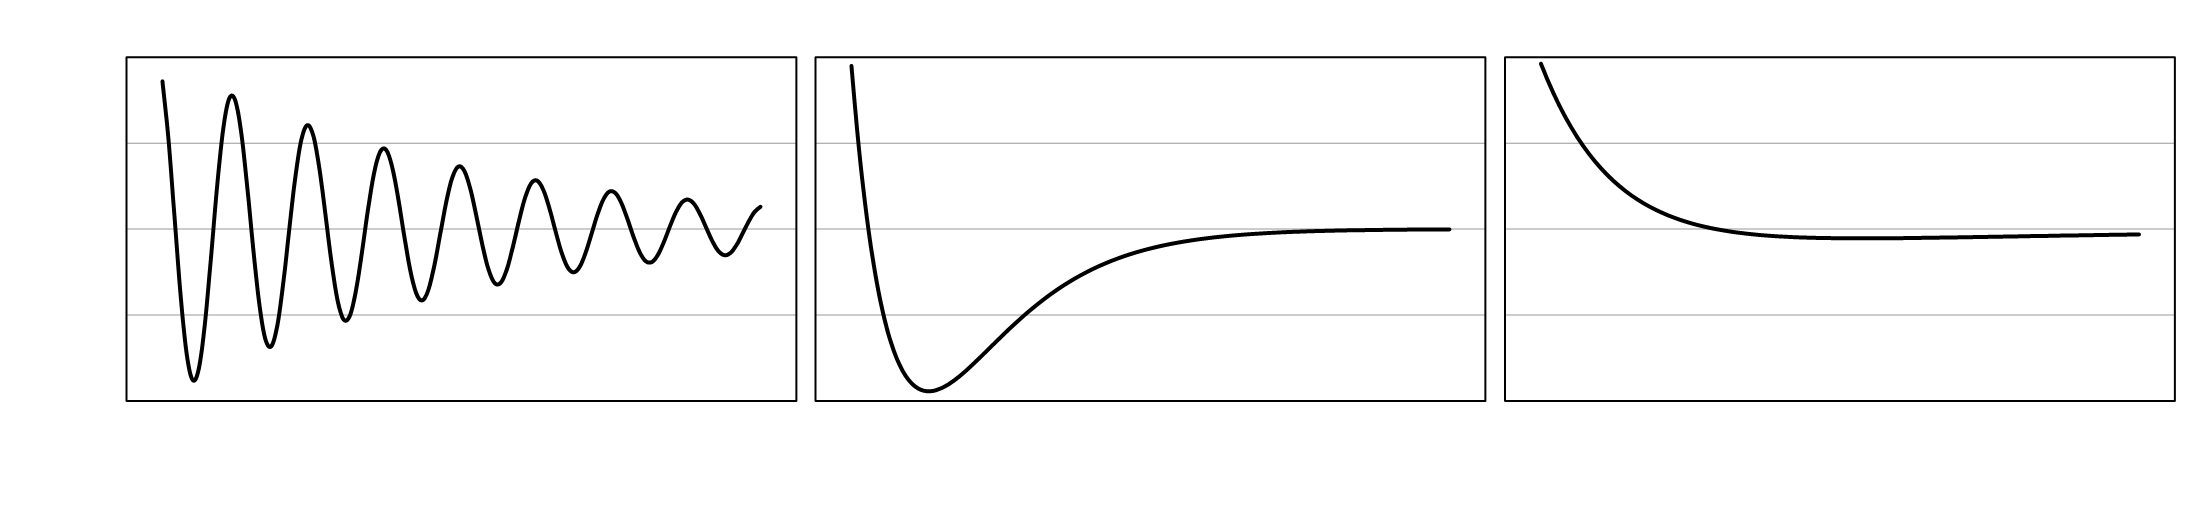
\includegraphics[width=14cm]{image/6-3-1.png}
	\caption{欠阻尼, 临界阻尼与过阻尼}
	\end{figure}

	\item \emph{过阻尼}(overdamped)

	此时$\beta>\omega_0$.\,从而振动和回复力被极大地抑制了.\,主要是一个在大阻力和初速度下缓慢回到平衡位置的运动.\,以上方程两根此时为两个正虚根:
	\[\omega_{1,2}=\ui(\beta\pm\sqrt{\beta^2-\omega_0^2})\]

	这样就得到了原阻尼振动方程的通解:
	\[x=\ue^{-\beta t}[A\ue^{\sqrt{\beta^2-\omega_0^2}t}+B\ue^{-\sqrt{\beta^2-\omega_0^2}t}]=C\ue^{-\beta t}\cosh(\sqrt{\beta^2-\omega_0^2}t+\varphi)\footnote{也有可能是$\sinh$}\]

	\item \emph{临界阻尼}(critical damped)

	这对应$\beta=\omega_0$的特殊情况.\,可以通过微分方程的理论,\,或者采用求$\beta\to \omega_0$极限的方式得到此时的运动方程.\,它为:
	\[x=\ue^{-\beta t}(A+Bt)\]

	临界阻尼在实际生活中的应用为:\,它是较快能够让振子回到平衡位置的理想阻尼大小.\,这一点不难理解,\,不难看出,\,欠阻尼情况的振幅随时间的衰减方式为$\ue^{-\beta t}$,\,也就是适当增大$\beta$有利于振幅尽快衰减.\,但是,\,过阻尼时,\,长时间后位移与时间的关系为
	\[x\sim \ue^{-\beta t}\cosh(\sqrt{\beta^2-\omega_0^2}t)\sim\ue^{-\beta t}\ue^{\sqrt{\beta^2-\omega_0^2}t}\sim \ue^{-\frac{\omega_0^2t}{\beta+\sqrt{\beta^2-\omega^2}}}\]

	这就不难发现,\,此时增加$\beta$只会使得$t$前的衰减系数变小而不利于尽快衰减其位移.\,从而,\,无论是欠阻尼还是过阻尼,\,临界阻尼是它们能够尽快回到平衡位置的极限.\,此时原来的固有频率对应的周期就是它回到平衡位置的特征时间.
\end{itemize}

对于欠阻尼情况,\,尤其是衰减因子$\beta<<\omega_0$的小阻尼情况,\,还有一些重要的性质值得挖掘.\,下面都默认是这样的前提:

\begin{wrapfigure}[17]{o}[-10pt]{7cm}
\centering
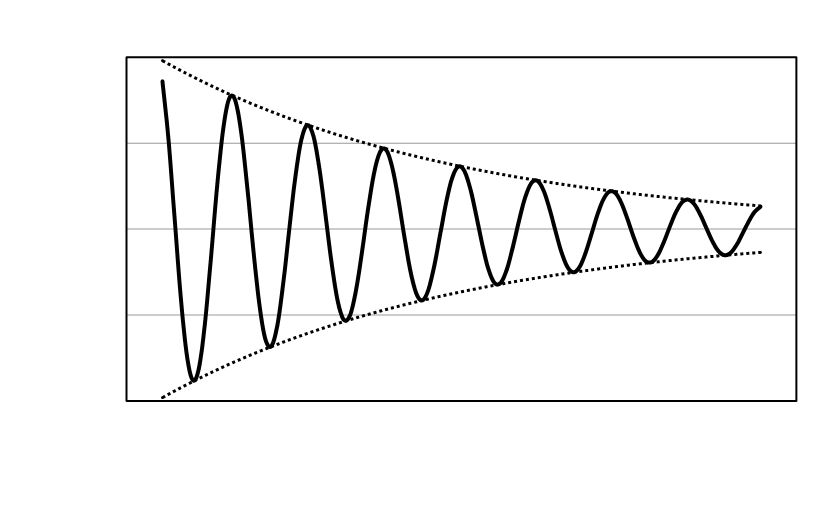
\includegraphics[width=7cm]{image/6-3-2.png}
\caption{\quad 小阻尼下的振幅衰减}
\end{wrapfigure}
从之前的运动方程解不难看出来,\,我们可以把小阻尼情况下的运动方程看作是一个振幅不断随着时间衰减的简谐振动.\,其振幅衰减函数和阻尼化角频率为:
\[A(t)=A_0\ue^{-\beta t}\]
\[\omega_d=\sqrt{\omega_0^2-\beta^2}\approx \omega_0\]

要讨论其衰减的原因,\,还有一种新的角度,\,便是考虑其能量.\,当振幅为$A$时,\,其动能,\,势能的和为:
\[E=T+V=\frac{1}{2}m\dot{x}^2+\frac{1}{2}kx^2\]

现在它不是守恒的,\,仅仅是在少数几个周期里面``近似''守恒.\,但是我们可以考虑求它在一个周期内的平均:
\[\bar{E}=\frac{1}{2}\cdot\frac{1}{2}m\omega_d^2 A^2+\frac{1}{2}\cdot\frac{1}{2} kA^2=\frac{1}{2}m\frac{\omega_0^2+\omega_d^2}{2} A^2\approx \frac{1}{2}m\omega_0^2 A^2\]

现在我们计算单位时间减少的能量的平均值.\,它其实就是阻尼造成的负功功率的平均值:
\[\bar{P}=\overline{\gamma v\cdot v}=\frac{1}{2}\gamma \omega_d^2 A^2\approx \frac{1}{2}\gamma \omega_0^2 A^2=\frac{1}{2}m \omega_0^2 A^2\cdot 2\beta\]

通过损耗功率等于能量的负导数,\,也可以得到振幅随着时间衰减的具体结果.\,我们现在关心一个重要的量,\,它实际上是反应振子振动单位相位所减少的能量占总能量的比例,\,我们把上式换一种写法:
\[\bar{P}=\frac{\omega_0\bar{E}}{Q}\]

以上引入的$Q$就是著名的\emph{品质因数}(quality factor).\,它越大,\,表示损耗越低,\,振子的阻尼就越小,\,就越接近``谐振''.\,实际上它算法为:
\[Q=\frac{\omega_0}{2\beta}\]

品质因数经常与另一个因子一起提出,\,两者是简单的导数关系,\,更精确地,\,我们定义:
\[\tan\delta=\frac{1}{Q}=\frac{2\beta}{\omega_0}\]

$\delta$被称作\emph{损耗角}(loss angle).\,一定要注意这两个概念是普遍的.\,谐振子模型是很多实际问题的抽象,\,它们作为谐振子都有自己的品质因数或损耗角,\,用以描述过程的一些共性,\,而且,\,不光可以用能量的损失的共性来定义品质因数和损耗角,\,还有很多重要的方式.\,详情见后.

\begin{wrapfigure}[17]{o}[-10pt]{7cm}
\centering
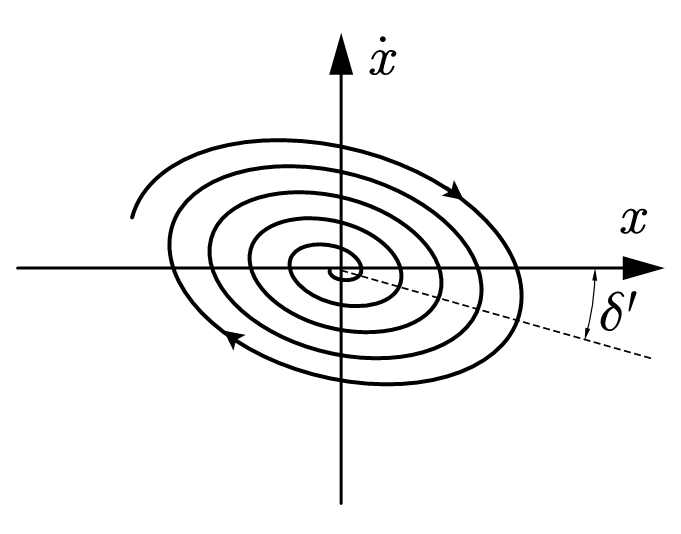
\includegraphics[width=7cm]{image/6-3-3.png}
\caption{阻尼振动的相图}
\end{wrapfigure}
现在我们来考虑简谐振动的\emph{相图}(phase diagram).\,在动力学中,\,这总是指把单个过程的运动,\,画成以其广义坐标和广义速度(或动量)为坐标轴的\emph{相空间}(phase space)中的曲线形成的图像.\,阻尼振动的代表性解为:
\[x=A\ue^{-\beta t}\ue^{\ui \omega_d t}\]

在这个解下,\,其速度为:
\[\dot{x}=(\ui\omega_d-\beta)A\ue^{-\beta t}\ue^{\ui \omega_d t}\]

两个量都在随时间衰减.\,从而在相图上就体现为一随着时间不断向着原点靠近的螺旋线.\,如果没有阻尼,\,那么标准简谐振动的相轨迹就是正椭圆:
\[\frac{x^2	}{A^2}+\frac{\dot{x}^2}{\omega_0^2A^2}=1\]

但是,\,有阻尼时除了是螺旋式的椭圆,\,它还不是``正''的.\,事实上,\,如果去除衰减因子,\,即将$x$和$\dot{x}$乘以个$\ue^{\beta t}$以抵消其衰减:
\[X=x\ue^{\beta t}=A\ue^{\ui \omega_d t}\quad,\quad V=\dot{x}\ue^{\beta t}=\ui(\omega_d+\ui\beta)A\ue^{\ui \omega_d t}\]

两者之间也不是恰好相差相位$\pi/2$,\,而是有一个额外相位差:
\[\Delta=\arctan\frac{\beta}{\omega_d}\]

%然而这个相位差也并不是相空间中的椭圆所倾斜的角度$\delta'$.\,为了得到倾角,\,我们可以先得到$X$与$V$形成的椭圆方程,\,为此取上式实部:
\[X=A\cos\omega_d t\quad,\quad V=-\omega_dA\sin\omega_d t-\beta A\cos \omega_d t\]
\[\Rightarrow \quad \omega_d^2X^2+(V+\beta X)^2=\omega_d^2 A^2\]
\[\Rightarrow \quad \omega_0^2 X^2+V^2+2\beta XV=\omega_d^2 A^2\]

为了求得顶点坐标,\,我们注意到对上式求偏导数就可以得到曲线上该点出的法向量:
\[\bs{n}=(\omega_0^2 X+\beta V\,,\,V+\beta X)\]

它需要与位矢$\bs{r}=(X\,,\,V)$共线,\,即:
\[\]


\section{多自由度小振动*}

\section{非线性摄动*}

\section{格波}



